\section{Inverse Gaussian sequence space model}\label{INTRO_IGSSM}

Let $\Xi$ be space of function from $[0, 1]$ to $\C$.
We equip the space with internal addition $+$ such that for any $x$ and $y$ in $\Xi$, $x + y = (t \mapsto x(t) + y(t))$, external product $\cdot$ such that for any $a$ in $\C$, $a \cdot x = (t \mapsto a \cdot x(t))$ and inner product $\langle x \vert y \rangle_{L^{2}} = \int x(t) \cdot \overline{y}(t) \d t$.
Hence, $\Xi$ equipped with the $L^{2}$-norm generated by $\langle \cdot \vert \cdot \rangle_{L^{2}}$ is a Hilbert space, for which the family of functions $(e_{s})_{s \in \Z}$ such that, for any $s$ in $\Z$, $e_{s} : t \mapsto \exp[- 2 \imath \pi s t]$ is an orthonormal basis.

Then, denote $\mathds{L}^{2}$ the sub-space of $\Xi$ of square integrable, \textbf{real-valued} functions defined on $[0, 1]$.
We define on $\mathds{L}^{2}$ the convolution product $\star$ such that for any $x$ and $y$ in $\mathds{L}^{2}$, we have $x \star y : t \mapsto \int_{[0, 1]} x(t - s - \lfloor t - s \rfloor) y(s) \d s$.
Let also be $\Theta$, the space of $\Z$-indexed, $\C$-valued sequences, equipped with internal addition $+$ such that for any $[x]$ and $[y]$ in $\Theta$, $[x] + [y] = (s \mapsto [x](s) + [y](s))$; external product $\cdot$ such that, for any $a$ in $\C$, $a \cdot [x] = (s \mapsto a \cdot [x](s))$; and inner product $\langle [x] \vert [y] \rangle_{l^{2}} = \sum_{s \in \Z} [x](s) \overline{[y]}(s)$.
Hence, $\Theta$ equipped with the $l^{2}$-norm derived from $\langle \cdot \vert \cdot \rangle_{l^{2}}$ is a Hilbert space, for which the family $(s \mapsto \mathds{1}_{\{s = s^{\star}\}})_{s^{\star} \in \Z}$ is an orthonormal basis.

In this context, we have $\mathcal{F}$, the Fourier transform with respect to $(e_{s})_{s \in \Z}$, that is to say, $\mathcal{F}: \Xi \to \Theta, \quad x \mapsto [x] (= s \mapsto \langle x \vert e_{s} \rangle_{L^{2}})$.
Notice that, for any element $x$ of $\mathds{L}^{2}$, due to the fact that it is real valued, we have for any $s$ in $\Z$, that $[x](s) = \overline{[x]}(-s)$, and due to the fact that it is square integrable, $[x]$ is square summable and we hence denote $\mathcal{L}^{2}$ the subspace of $\Theta$ of square summable sequences $[x]$ such that, for any $s$ in $\Z$, $[x](s) = \overline{[x]}(-s)$.
Also, for any $x$ and $y$ in $\mathds{L}^{2}$, we have $[x \star y] = [x] \cdot [y]$.
Due to the fact that the Fourier transform is unitary, we also have, for any $t$ in $[0, 1]$ and $x$ in $\mathds{L}^{2}$ that $x(t) = \mathcal{F}^{\star}([x]) = \sum_{s \in \Z} [x](s) e_{s}(t)$.

\medskip

Keeping in mind the notations used until here, let $f$ and $h$ be in $\mathds{L}^{2}$ and $g := f \star h$, hence, we have $T : \mathds{L}^{2} \to \mathds{L}^{2}, \quad x \mapsto x \star h$ and we have three elements of $\mathcal{L}^{2}$ given by, $\theta^{\circ} = \mathcal{F}(f)$, $\lambda = \mathcal{F}(h)$, and $\phi = \mathcal{F}(g) = \theta^{\circ} \cdot \lambda$.
Remind that for any $x$ in $\mathds{L}^{2}$, we have $\Vert x \Vert_{L^{2}} = \Vert [x] \Vert_{l^{2}}$ and hence we will study estimation procedures for $\theta^{\circ}$, however, the reader should keep in mind that it is motivated by the estimation of $f$, which has equivalent performances due to Plancherel theorem.

\subsection{Known operator}
Let $Y$ be the Gaussian process such that for any $t$ in $[0, 1]$, we have $\d Y(t) = \d W(t) + g(t) \d t$ where $W$ is the Brownian motion.
Hence, there exist sequences of real-valued random variables $(\xi_{1}(s))_{s \in \Z}$ and $(\xi_{2}(s))_{s \in \Z}$ such that for any $s$ and $s'$ in $\Z$, we have $\int_{[0, 1]} e_{s}(t) \d Y(t) = \int_{[0, 1]} \cos(2 \pi s t) \d W(t) + \imath \int_{[0, 1]} \sin(2 \pi s t) \d W(t) + \phi(s) = \xi_{1}(s) + \imath \xi_{2}(s) + \phi(s)$ with $\xi_{1}(s) \sim \mathcal{N}(0, 1/2)$, $\xi_{2}(s) \sim \mathcal{N}(0, 1/2)$, and $\xi_{1}(s)$ is independent of $\xi_{2}(s)$, in addition, $\Cov(\xi_{1}(s), \xi_{1}(s')) = \mathds{1}_{\{\vert s' \vert = \vert s \vert\}}$ and $\Cov(\xi_{2}(s), \xi_{2}(s')) = \text{Sign}(s \cdot s') \mathds{1}_{\{\vert s' \vert = \vert s \vert\}}$.

\medskip

Define the \iid stochastic process $(Y_{p})_{p \in \Z}$ such that, for any $p$ in $\Z$, $Y_{p}$ is identically distributed to $Y$.
We observe the sub-vector $Y^{n} = (Y_{p})_{p \in \llbracket 1, n \rrbracket}$ of $(Y_{p})_{p \in \Z}$ and define, for any $s$ in $\N$ the estimates $\phi_{n}(s) = \sum_{p = 1}^{n} \int_{[0, 1]} e_{s}(t) \d Y(t) / n$ which verifies $\Re(\phi_{n}(s)) \sim \mathcal{N}(\Re(\phi(s)), 2/n)$ and $\Im(\phi_{n}(s)) \sim \mathcal{N}(\Im(\phi(s)), 2/n)$ and as we assume \nref{AS_INTRO_DATA_KNOWN}, we know $\lambda$ and for any $s$ in $\Z$ $\vert \lambda(s) \vert > 0$ so we can define $\theta_{n}(s) := \phi_{n}(s) / \lambda(s)$, which verifies $\Re(\theta_{n}(s)) \sim \mathcal{N}(\Re(\theta^{\circ}), \Lambda(s)/n)$; $\Im(\theta_{n}(s)) \sim \mathcal{N}(\Im(\theta^{\circ}), \Lambda(s)/n)$; and $\Cov(\Re(\theta_{n}(s)), \Im(\theta_{n}(s))) = 0$.
Finally, we define, for any $m$ in $\N$, the projections estimator $\theta_{n, \overline{m}} = (\theta_{n}(s) \mathds{1}_{\{\vert s \vert \leq m\}})_{s \in \Z}$.
We give, in \nref{igssm:estimation} an illustration of a projection estimator.

\begin{figure}
  \centering
  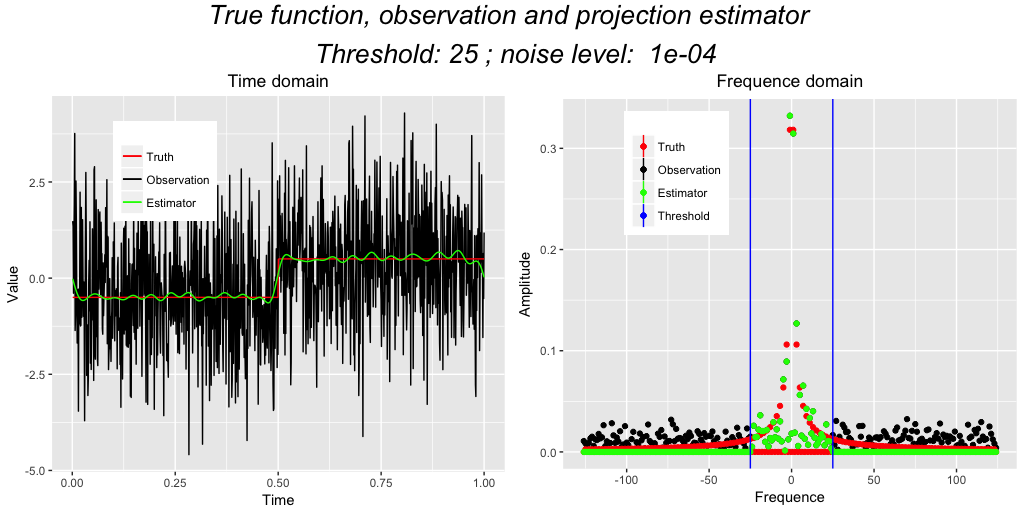
\includegraphics[width=1.\linewidth]{gauss/estimation/frequentist.png}
  \caption{Projection estimator in the time and frequency space, direct problem case.}
\label{igssm:estimation}
\end{figure}

Notice that, for any $m$ in $\N$, $\E[\Vert \theta^{\circ} - \theta_{n, \overline{m}} \Vert_{l^{2}}^{2}] = 2 \sum_{s \in \N} \E[(\Re(\theta^{\circ}(s)) - \Re(\theta_{n, \overline{m}}(s)))^{2}] + 2 \sum_{s \in \N} \E[(\Im(\theta^{\circ}(s)) - \Im(\theta_{n, \overline{m}}(s)))^{2}]$.
Hence, real and imaginary parts can be treated separately in an identical manner and considering the positive indexes is sufficient and we only will give attention to the estimation of the real part of the positively indexed coefficients of $\theta^{\circ}$ and we give this final formulation for the model.

\begin{de}\label{INTRO_IGSSM_DE}
Let $\Theta$ be the space of $\N^{\star}$-indexed, $\R$-valued sequences, equipped with the inner product $\langle \cdot \vert \cdot \rangle_{l^{2}} : ([x], [y]) \mapsto \sum_{s \in \N} [x](s) \cdot [y](s)$ and the associated norm $\Vert \cdot \Vert_{l^{2}}: [x] \mapsto \sum[x](s)^{2}$.
Let $\mathcal{L}^{2}$ be the subspace of $\Theta$ of square-summable sequences.

Given three elements of $\Theta$ denoted $\theta^{\circ}$, $\lambda$, and $\phi$, such that, $\phi = \theta^{\circ} \cdot \lambda$; for any $s$ in $\N$, $0 < \vert \lambda(s) \vert \leq 1$; and $\theta^{\circ}$ is an element of $\mathcal{L}^{2}$.

We observe $\phi_{n}$ in $\Theta$ such that, for any $s$ and $s'$ in $\N$ such that $s \neq s'$, we have $\phi_{n}(s) \sim \mathcal{N}(\phi(s), n^{-1})$ and $\Cov(\phi_{n}(s), \phi_{n}(s')) = 0$.
\assEnd
\end{de}

The likelihood for this model is given by
\[L(\phi_{n}, \theta) \propto \exp[n^{-1}(\sum\nolimits_{s \in \N} \phi_{n}(s) \theta(s) \lambda(s) - \sum\nolimits_{s \in \N} \Lambda(s)^{-1}\theta(s)^{2}/2)].\]

Notice that as in \nref{as:il}, $\V[\langle Y_{0}\vert e_{s} \rangle_{L^{2}}] = 1$, hence, all the results obtained considering the convergence rates remain true.
Hence let us give the following reminders.

\begin{nota*}
For any $m$ in $\mathds{N}^{\star}$; $s$ in $\mathds{N}^{\star}$; and $\theta$ in $\Theta$, let be the following quantities:
\begin{multline*}
\b_{m}^{2}(\theta) := \Vert \theta_{\underline{0}}\Vert_{l^{2}}^{-2} \Vert \theta_{\underline{m}} \Vert^{2}; \quad \Lambda(s) = \vert \lambda^{-1}(s) \vert^{2};\\
\Lambda_{\circ}(m) = m^{-1} \sum\nolimits_{0 < s \leq m} \Lambda(s); \quad \Lambda_{+}(m) := \max\nolimits_{s \in \llbracket 1, m \rrbracket}\{\Lambda(s)\}.
\end{multline*}
We then denote in the following way the risk for projection estimators:
\begin{equation*}
\mathcal{R}_{n}^{m}(\theta^{\circ}, \Lambda) := [n^{-1} m \Lambda_{\circ}(m) \vee \b_{m}^{2}(\theta^{\circ})].
\end{equation*}
Which gives us the following oracle rates,
\begin{multline*}
m^{\circ}_{n} \in \argmin\nolimits_{m \subset \mathds{M}}\left\{\mathcal{R}_{n}^{m}(\theta, \lambda)\right\} =  \argmin\nolimits_{m \subset \mathds{M}}\left\{[n^{-1} m \Lambda_{\circ}(m) \vee \b_{m}^{2}(\theta^{\circ})]\right\};\\
\mathcal{R}_{n}^{\circ}(\theta^{\circ}, \Lambda) = \mathcal{R}_{n}^{m_{n}^{\circ}}(\theta^{\circ}, \Lambda) = \min\nolimits_{m \in \N}\mathcal{R}_{n}^{m}(\theta^{\circ}, \Lambda).
\end{multline*}
And we were able to obtain the following maximal rates.
\begin{multline}
 \dRa{\Di}{\xdfCw[],\Lambda}:=[\xdfCw^2\vee\Di\oiSv \ssY^{-1}]:=\max\big(\xdfCw^2,\Di \oiSv \ssY^{-1}\big),\\
\hfill \mnDi(\xdfCw[]):=\mnDi(\xdfCw[],\Lambda):=\argmin\Nset[{\Di\in\N}]{\dRa{\Di}{\xdfCw[],\Lambda}}\quad\text{ and }\hfill\\\mnRa{\xdfCw[],\Lambda}:=\dRa{\mnDi({\xdfCw[]})}{\xdfCw[],\Lambda}=\min\Nset[{\Di\in\N}]{\dRa{\Di}{\xdfCw[],\Lambda}}.
\end{multline}
\assEnd
\end{nota*}

\begin{figure}
  \centering
  \begin{tabular}{@{}c@{}}
    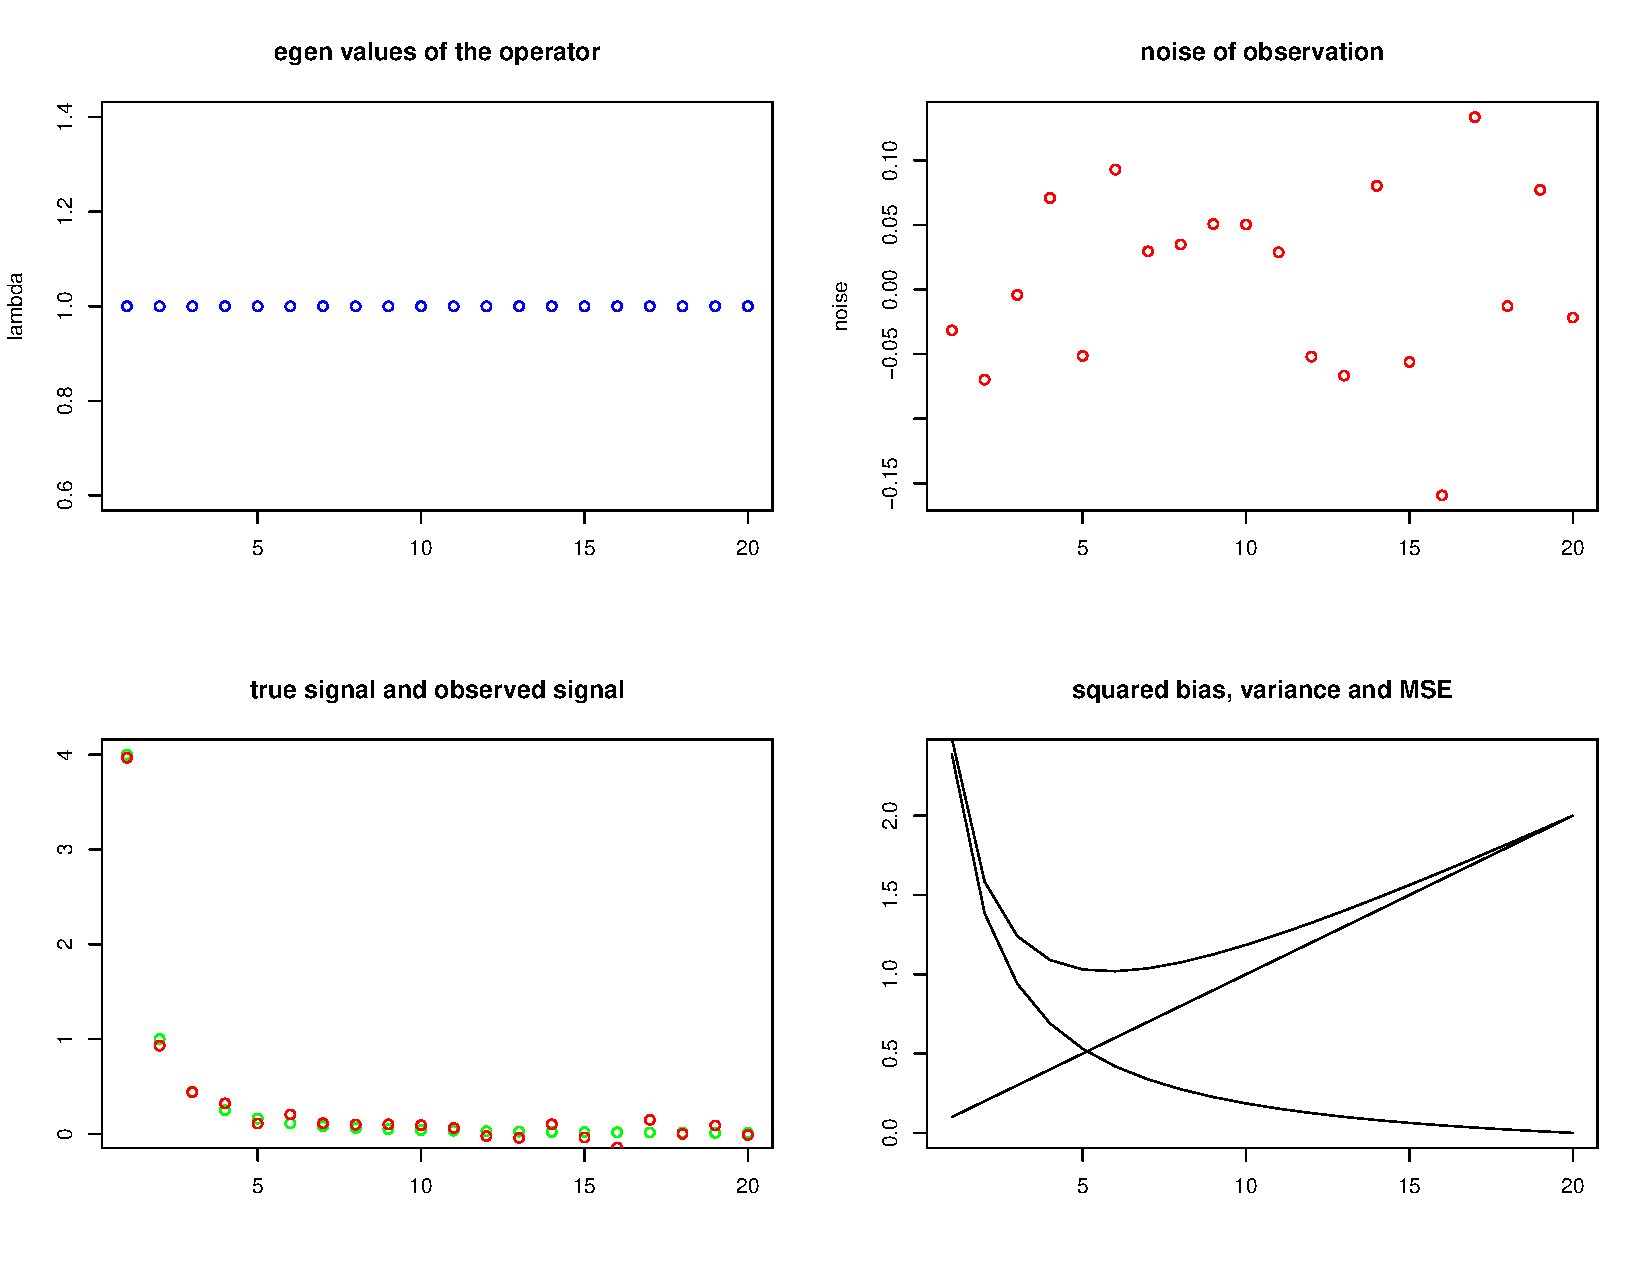
\includegraphics[width=.49\linewidth]{general/direct-case.pdf} \\[\abovecaptionskip]
  \end{tabular}
  \begin{tabular}{@{}c@{}}
    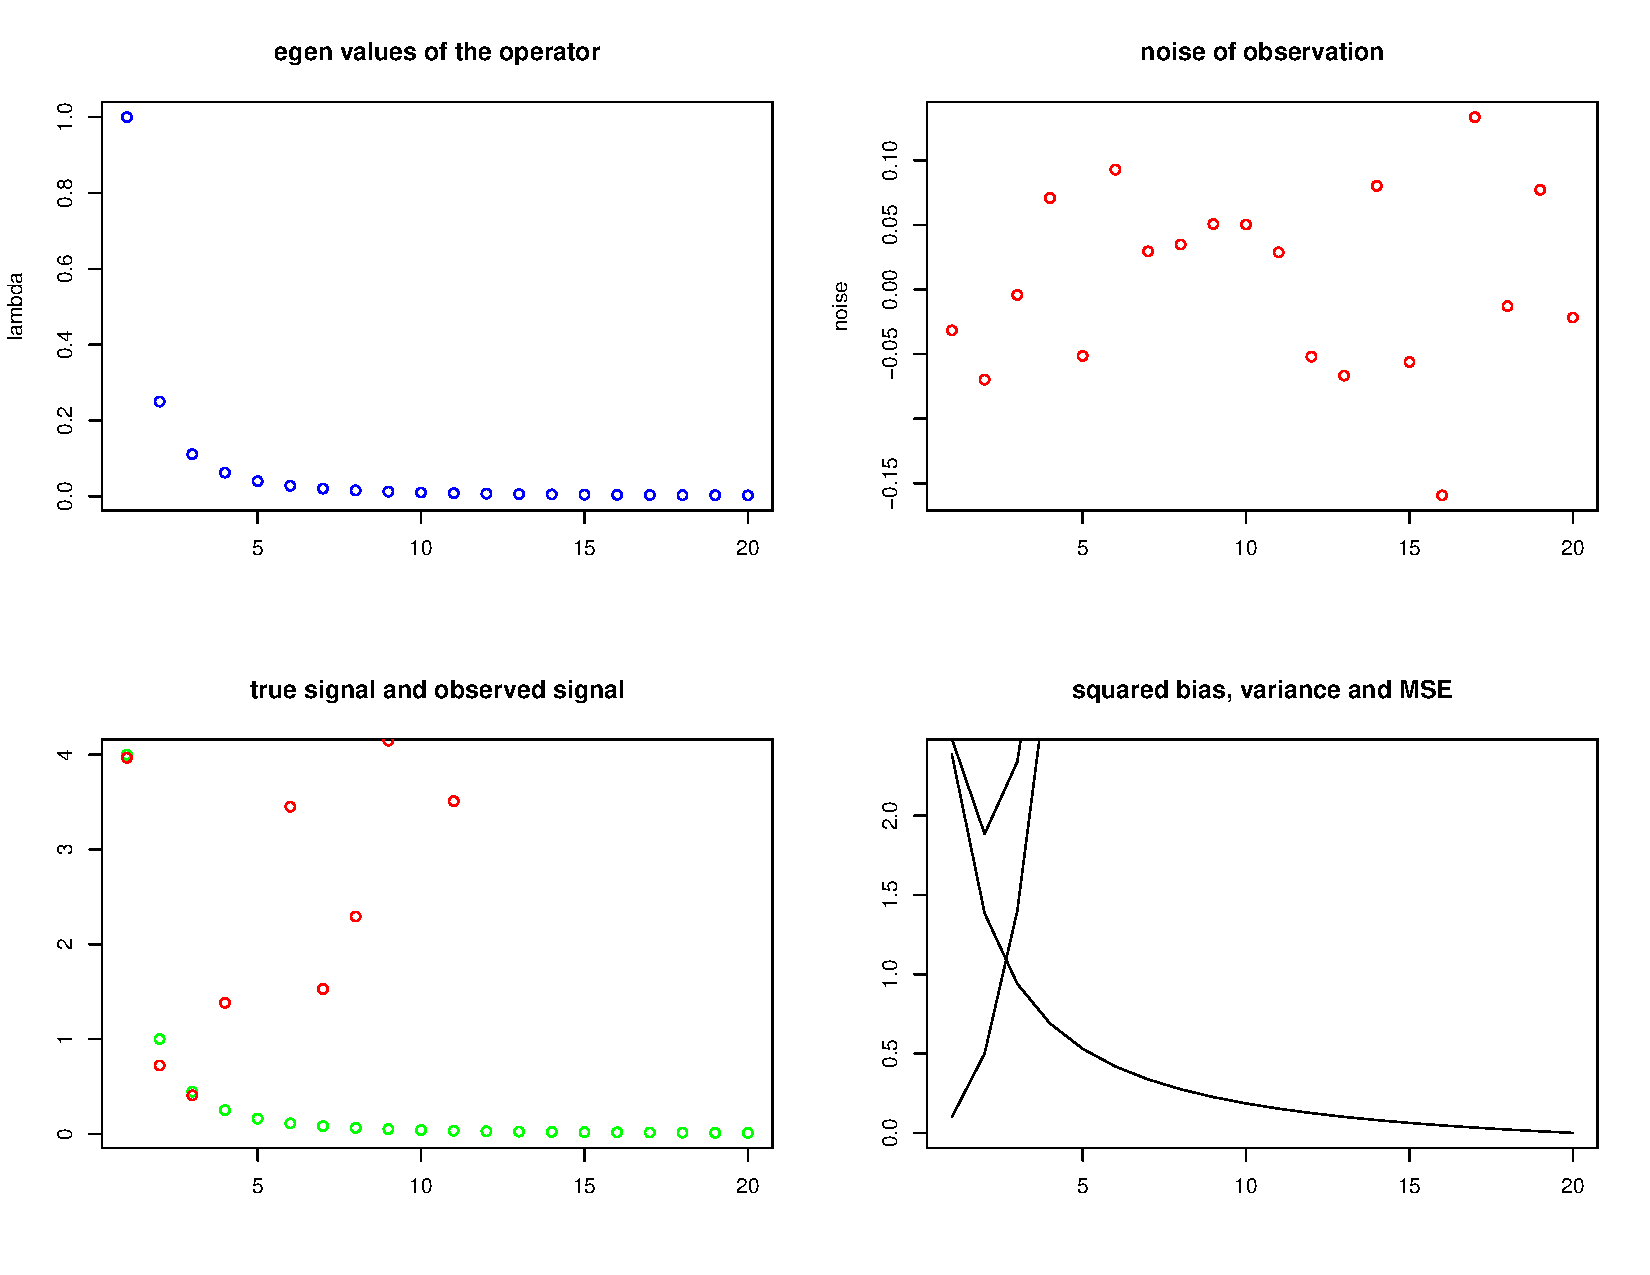
\includegraphics[width=.49\linewidth]{general/mildly-illposed.pdf} \\[\abovecaptionskip]
  \end{tabular}
  \caption{Influence of the operator Eigen-values sequence decay on the quadratic risk}\label{igssm:mildsev}
\end{figure}

\begin{rem*}
We shall emphasise that $\oRa{\xdf,\Lambda}\geq \ssY^{-1}$ for all
  $\ssY\in\N$, and
  
  $\lim_{n \rightarrow \infty} \oRa{\xdf,\Lambda}=0$.
  Observe that for all $\delta>0$ there exists $\Di_{\delta}\in\N$ and
  $\ssY_\delta\in\N$ such that for all $\ssY\geq \ssY_{\delta}$ holds
  $\bias[\Di_\delta]^2(\xdf)\leq \delta$ and
  $\Di_{\delta} \oiSv[\Di_\delta] \ssY^{-1}\leq\delta$, and whence
  $\oRa{\xdf,\Lambda}\leq\dRa{\Di_\delta}{\xdf,\Lambda}\leq \delta$.
  Moreover, we have $\oDi{\ssY}\in\nset{1,\ssY}$. Indeed, by construction
  holds
  $\bias[\ssY]^2(\xdf)\leq 1<(\ssY+1)\ssY^{-1}\leq
  (\ssY+1)\oiSv[\ssY+1]{}\ssY^{-1}$, and hence
  $\dRa{\ssY}{\xdf,\Lambda}<\dRa{\Di}{\xdf,\Lambda}$ for all
  $\Di\in \nsetro{\ssY+1,\infty}$ which in turn implies the claim
  $\oDi{\ssY}\in\nset{1,\ssY}$. Obviously, it follows thus
  $\oRa{\xdf,\Lambda}=\min\set{ \dRa{\Di}{\xdf,\Lambda}
    ,\Di\in\nset{1,\ssY}}$ for all $\ssY\in\N$. We shall use those
  elementary findings in the sequel without further reference.
The sequence $\mathcal{R}_{n}^{\circ}(\theta, \lambda)$ is then an exact oracle convergence rate and the projection estimator $\theta_{n, \overline{m_{n}^{\circ}}}$ is an oracle optimal estimator.

\medskip

Note that, in case \ref{oo:xdf:p}, the oracle rate is parametric, that is
$\oRa{\xdf, \Lambda} \approx \ssY^{-1}$. More precisely, if $\xdf=0$ then
for each  $\Di\in\N$,
$\E\Vnormlp{\txdfPr-\xdf}^2=\Di\oiSv[\Di]\ssY^{-1}$,
and hence $\oDi{\ssY}=1$ and $\oRa{\xdf, \Lambda}=2\oiSv[1]\ssY^{-1}\sim\ssY^{-1}$. Otherwise
if there is $K\in\N$  with $\bias[K-1](\xdf)>0$ and
$\bias[K](\xdf)=0$, then setting
$\ssY_{\xdf}:=\tfrac{K\oiSv[K]}{\bias[K-1]^2(\xdf)}$, for all
$\ssY\geq \ssY_{\xdf}$ holds
$\bias[K-1]^2(\xdf)>K\oiSv[K]\ssY^{-1}$, and hence  $\oDi{\ssY}=K$ and
$\oRa{\xdf,\Lambda}= K\oiSv[K]\ssY^{-1}\sim \ssY^{-1}$.
On the other hand side, in case \ref{oo:xdf:np} the oracle rate is
non-parametric, more precisely, it holds
$\lim_{\ssY\to\infty}\ssY\oRa{\xdf,\Lambda}=\infty$. Indeed, since
$\bias[\oDi{\ssY}]^2(\xdf)\leq\oRa{\xdf,\Lambda}=\oRa{\xdf,\Lambda}\in\mathfrak{o}_{n}(1)$ follows $\oDi{\ssY}\to\infty$ and hence
$\oDi{\ssY}\oiSv[\oDi{\ssY}]\to\infty$ which implies the claim because
$\ssY\oRa{\xdf,\Lambda}\geq\oDi{\ssY}\oiSv[\oDi{\ssY}]$.

\medskip

When considering the maximal rate, by construction it holds 
$\mnRa{\xdfCw[],\Lambda}\geq \ssY^{-1}$ for all $\ssY\in\N$.
The following statements can be
shown using the same arguments as in \nref{oo:rem:ora}
by exploiting that the sequence $\xdfCw[]$ is assumed to be
non-increasing, strictly positive with limit zero and $\xdfCw[(1)]=1$. 
Thereby, we conclude that 
$\mnRa{\xdfCw[],\Lambda}=\mathfrak{o}_{n}(1)$ and $\ssY\mnRa{\xdfCw[],\Lambda}\to\infty$ as well as 
$\mnDi(\xdfCw[])\in\nset{1,\ssY}$ for all $\ssY\in\N$. It follows also that
$\mnDi(\xdfCw[])=\argmin\Nset[{\Di\in\nset{1,n}}]{\dRa{\Di}{\xdfCw[],\Lambda}}$ and 
$\mnRa{\xdfCw[],\Lambda}=\min\Nset[{\Di\in\nset{1,n}}]{\dRa{\Di}{\xdfCw[],\Lambda}}$ for all
$\ssY\in\N$. We shall stress that in this situation the rate
$\mnRa{\xdfCw[],\Lambda}$ is non-parametric.
\remEnd
\end{rem*}

We give in \nref{igssm:oracle} an illustration of the oracle estimator in a Gaussian sequence space model, in the direct problem case that is to say $\lambda(s) = 1$ for all $s$ in $\N$.

\begin{figure}
  \centering
  \begin{tabular}{@{}c@{}}
    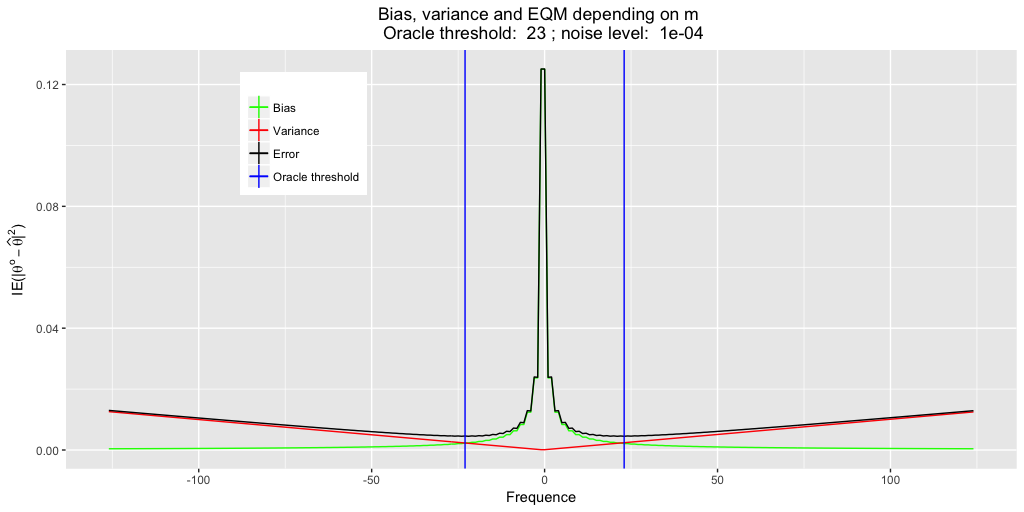
\includegraphics[width=.49\linewidth]{gauss/error/oracle_threshold.png} \\[\abovecaptionskip]
  \end{tabular}
  \begin{tabular}{@{}c@{}}
    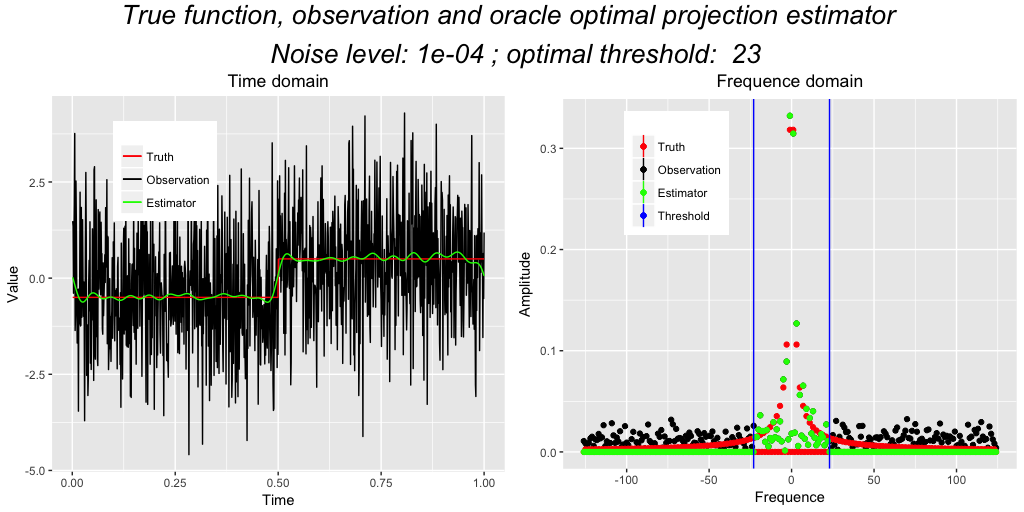
\includegraphics[width=.49\linewidth]{gauss/error/oracle_estimator.png} \\[\abovecaptionskip]
  \end{tabular}
  \caption{Illustration of the oracle value for $m$ and associated projection estimator.}\label{igssm:oracle}
\end{figure}

\subsection{Unknown operator}
In the case of an unknown operator, that is, $h$, and hence, $\lambda$ unknown, we supposed that, in addition to $Y$ we define another Gaussian process $\epsilon$.
Let $\epsilon$ be the Gaussian process such that for any $t$ in $[0, 1]$, we have $\d \epsilon(t) = \d W(t) + h(t) \d t$ where $W$ is the Brownian motion.
Hence, there exist sequences of real-valued random variables $(\xi_{3}(s))_{s \in \Z}$ and $(\xi_{4}(s))_{s \in \Z}$ such that for any $s$ and $s'$ in $\Z$, we have $\int_{[0, 1]} e_{s}(t) \d \epsilon(t) = \int_{[0, 1]} \cos(2 \pi s t) \d W(t) + \imath \int_{[0, 1]} \sin(2 \pi s t) \d W(t) + \lambda(s) = \xi_{3}(s) + \imath \xi_{4}(s) + \phi(s)$ with $\xi_{3}(s) \sim \mathcal{N}(0, 1/2)$, $\xi_{4}(s) \sim \mathcal{N}(0, 1/2)$, and $\xi_{3}(s)$ is independent of $\xi_{4}(s)$, in addition, $\Cov(\xi_{3}(s), \xi_{3}(s')) = \mathds{1}_{\{\vert s' \vert = \vert s \vert\}}$ and $\Cov(\xi_{4}(s), \xi_{4}(s')) = \text{Sign}(s \cdot s') \mathds{1}_{\{\vert s' \vert = \vert s \vert\}}$.
Define the \iid stochastic process $(\epsilon_{p})_{p \in \Z}$ such that, for any $p$ in $\Z$, $\epsilon_{p}$ is identically distributed to $\epsilon$.
We observe the sub-vector $\epsilon^{n_{\lambda}} = (\epsilon_{p})_{p \in \llbracket 1, n_{\lambda} \rrbracket}$ of $(\epsilon_{p})_{p \in \Z}$ and define, for any $s$ in $\N$ the estimates

$\lambda_{\ssE}(s) = \sum_{p = 1}^{n_{\lambda}} \int_{[0, 1]} e_{s}(t) \d \epsilon(t) \ssE^{-1}$ which verifies $\Re(\lambda_{\ssE}(s)) \sim \mathcal{N}(\Re(\lambda(s)), 2\ssE^{-1})$ and $\Im(\lambda_{\ssE}(s)) \sim \mathcal{N}(\Im(\lambda(s)), 2 \ssE^{-1})$ so we define $\theta_{\ssY, \ssE}(s) := \phi_{n}(s) \lambda_{\ssE}^{+}(s)$, with $\lambda_{\ssE}^{+}(s) = \lambda_{\ssE}^{-1}(s) \mathds{1}_{\{\vert \lambda_{\ssE}\vert^{2} \geq \ssE^{-1}\}}$.

We may carry the same observations about the convergence rate and hence we give the following final definition for the model in the case of unknown operator.
\begin{de}\label{INTRO_IGSSM_DE_UK}
Let $\Theta$ be the space of $\N$-indexed, $\R$-valued sequences, equipped with the inner product $\langle \cdot \vert \cdot \rangle_{l^{2}} : ([x], [y]) \mapsto \sum_{s \in \N} [x](s) \cdot [y](s)$ and the associated norm $\Vert \cdot \Vert_{l^{2}}: [x] \mapsto \sum[x](s)^{2}$.
Let $\mathcal{L}^{2}$ be the subspace of $\Theta$ of square-summable sequences.

Given three elements of $\Theta$ denoted $\theta^{\circ}$, $\lambda$, and $\phi$, such that, $\phi = \theta^{\circ} \cdot \lambda$; for any $s$ in $\N$, $0 < \vert \lambda(s) \vert \leq 1$; and $\theta^{\circ}$ is an element of $\mathcal{L}^{2}$.

We observe the $\Theta$-valued random variable $\phi_{n}$  such that, for any $s$ and $s'$ in $\N$ such that $s \neq s'$, we have $\phi_{n}(s) \sim \mathcal{N}(\phi(s), n^{-1})$ and $\Cov(\phi_{n}(s), \phi_{n}(s')) = 0$.
On the other hand, we also observe the $\Theta$-valued random variable $\lambda_{\ssE}$ such that, for any $s$ and $s'$ in $\N$ such that $s \neq s'$, we have $\lambda_{\ssE}(s) \sim \mathcal{N}(\lambda(s), \ssE^{-1})$ and $\Cov(\lambda_{\ssE}(s), \lambda_{\ssE}(s')) = 0$.
\assEnd
\end{de}

As a direct consequence we have for any $s$ in $\N^{\star}$, as in \nref{as:il}, $\lambda(s) - \lambda_{\ssE}(s) \sim \mathcal{N}(0, \ssE^{-1})$ and hence, $\ssE^{2} \E\vert \lambda(s) - \lambda_{\ssE}(s) \vert^{4} = 3$ and $n_{\lambda} \E[\vert \lambda_{\ssE}(s) - \lambda(s) \vert^{2}] = 1$.
Hence, \nref{as:il} holds true and the analysis of the optimal rates carried out previously still holds true.
We hence remind the following results we obtained.

\begin{nota*}
In addition to the case of a known operator, we defined the following rate, for all $\ssE$ in $N$
\begin{multline*}
\mathcal{R}_{n_{\lambda}}^{\dagger}(\theta^{\circ}, \Lambda) := \sum_{s \in \mathds{F}}\vert \theta(s) \vert^{2} (1 \wedge n_{\lambda}^{-1} \Lambda(s))\\
\mmRa{\xdfCw[],\Lambda}:=\max_{s\in\N}\{\xdfCw[(s)]^2[1\wedge \iSv[s]/\ssE]\}\Vnorm[1/{\xdfCw[]}]{\xdf}^2.
\end{multline*}
\end{nota*}

\begin{rem*}
We have
\begin{equation*}
\mathcal{R}_{n, n_{\lambda}}(\theta_{n, n_{\lambda}, \overline{m_{n}^{\circ}}}) \leq (1 + \Vert \theta^{\circ}_{\underline{0}} \Vert_{l^{2}}^{2})\mathcal{R}_{n}^{\circ}(\theta^{\circ}, \Lambda) + 2 \mathcal{R}_{n_{\lambda}}^{\dagger}(\theta^{\circ}, \Lambda).
\end{equation*}
We note that $\Vnormlp{\xdf_{\underline{0}}}^2=0$ implies
  $\mRa{\xdf,\Lambda}=0$, while for $\Vnormlp{\xdf_{\underline{0}}}^2>0$ holds
  $\mRa{\xdf,\Lambda}\geq \sum_{s:\iSv[s]>\ssE} \vert \fxdf[(s)] \vert ^2+\ssE^{-1}\sum_{s:\iSv[s]\leq\ssE} \vert \fxdf[(s)] \vert ^2  \geq\ssE^{-1}\sum_{s\in\N} \vert \fxdf[(s)] \vert ^2=\Vnormlp{\xdf_{\underline{0}}}^2
  \ssE^{-1}$, thereby whenever $\xdf\ne 0$
  any additional term of order $\ssY^{-1}+\ssE^{-1}$
  is negligible with respect to the rate
  $\oRa{\xdf,\Lambda}+\mRa{\xdf,\Lambda}$, since
  $\oRa{\xdf,\Lambda}\geq \ssY^{-1}$, 
  which we will use below without further reference. We shall
  emphasise that in case $\ssY=\ssE$ it holds
  \begin{multline}
    \mRa[\ssY]{\xdf,\Lambda}=\sum_{0 < s \leq m_{n}^{\circ}} \vert \fxdf[(s)] \vert^2 [1 \wedge \ssY^{-1}\iSv[s]]
    + \sum_{s > m_{n}^{\circ}} \vert \fxdf[(s)] \vert ^2[1\wedge\ssY^{-1}\iSv[s]]\\
    \leq \cst{}\Vnormlp{\xdf_{\underline{0}}}^2 \ssY^{-1} \oDi{\ssY}
    \oiSv[\oDi{\ssY}] +
    \cst{}\Vnormlp{\xdf_{\underline{0}}}^2\bias[\oDi{\ssY}]^2(\theta^{\circ})\leq
    \Vnormlp{\xdf_{\underline{0}}}^2\dRa{\oDi{\ssY}}{\xdf,\Lambda}
  \end{multline}
  which in turn implies $\mathcal{R}_{n, n_{\lambda}}(\theta_{n, n_{\lambda}, \overline{m_{n}^{\circ}}}) \leq 4 \Vert \theta^{\circ}_{\underline{0}} \Vert_{l^{2}}^{2}\mathcal{R}_{n}^{\circ}(\theta^{\circ}, \Lambda)$.
  In other words, the estimation of the unknown operator $T$ is negligible whenever $\ssY\leq\ssE$.
  
  \medskip
  
Considering then the behaviour of the oracle rate, we have the following results.
We note that in case \ref{oo:xdf:p}
$\mRa{\xdf,\Lambda}\leq
\Vnormlp{\xdf_{\underline{0}}}^2\miSv[K]\ssE^{-1}$
and hence
\begin{equation}
 \nmRi{\hxdfPr[\oDi{\ssY}]}{\xdf,\Lambda}
 % \FuEx\Vnormlp{\hxdfPr[\oDi{\ssY}]-\xdf}^2
 \leq
\{[1\vee\Vnormlp{\xdf_{\underline{0}}}^2]\{
K\oiSv[K]\ssY^{-1}+\miSv[K]\ssE^{-1}\}
\end{equation}
for all $\ssE\in\N$ and $\ssY\geq\ssY_{\xdf}$ with $\ssY_{\xdf}$ as in \nref{oo:rem:ora}. In other words the
rate is parametric in both the $\rE$-sample size $\ssE$ and the $\rY$-sample size $\ssY$. Thereby, the  additional estimation of $\lambda$ is negligible whenever $\ssE\geq\ssY$.  In the
opposite case \ref{oo:xdf:np}, it is obviously of interest to characterise the minimal size $\ssE$ of the additional
sample from $\rE$ needed to attain the same rate as in case of a known
operator. We carried this discussion in \nref{ge:il:oo:kn}.

\medskip

On the other hand, if one is interested in the maximal risk, we have the following results.
For all $\ssE\in\N$ holds
$\sup_{\xdf\in\rwCxdf}\oRa{\xdf,\Lambda}\leq
\xdfCr^2\mmRa{\xdfCw[],\Lambda}$, since for all
$\xdf\in\rwCxdf$ 
\begin{equation}
  \mmRa{\xdf,\Lambda}=\sum_{s\in\N^{\star}} \vert \fxdf[(s)] \vert ^2[1\wedge \iSv[s]/\ssE]\leq
\max_{s\in\N}\{\xdfCw[(s)]^2\min(1,\iSv[s]/\ssE)\}\Vnorm[1/{\xdfCw[]}]{\xdf}^2.
\end{equation}
It follows for all $\Di,\ssY,\ssE\in\N$ immediately that 
\begin{equation}
  \nmRi{\hxdfPr}{\rwCxdf,\Lambda}
  \leq (\xdfCr^2+8) \dRa{\Di}{\xdfCw[],\Lambda}+16\xdfCr^2\mmRa{\xdfCw[],\Lambda}.
\end{equation}
The upper bound in the last display depends on the dimension parameter
$\Di$ and hence by choosing an optimal value $\mnDi$ as in
\eqref{mm:de:nra} the upper bound
will be minimised, that is
\begin{equation}
  \nmRi{\hxdfPr[\mnDi]}{\rwCxdf,\Lambda}
  \leq (\xdfCr^2+8) \mnRa{\xdfCw[],\Lambda}+16\xdfCr^2\mmRa{\xdfCw[],\Lambda}.
\end{equation}

\medskip

 Since the operator $T$ is not known, it is natural to
  consider a maximal risk also over a class for $\edf$ characterising the behaviour of
  $\Nsuite[s]{\iSv[s]= \vert \fedf[(s)] \vert ^{-2}}$, precisely $\rwCedf:=\{\edf\in\lp[2]:\edfCr^{-2}\leq\edfCw[s] \vert \fedf[(s)] \vert ^{2}=
\edfCw[s]\iSv[ s ]^{-1}\leq \edfCr^{2},\;\forall s\in\N^{\star}\}$.
We shall note that for all $\Di\in\N$ and any $\edf\in\rwCedf$,
$\edfCr^{-2}\leq\miSv/\edfCwm\leq \edfCr^{2}$,
$\edfCr^{-2}\leq\oiSv/\edfCwo\leq \edfCr^{2}$. Setting
for all $\ssY,\ssE\in\N$
\begin{multline}
 \dRa{\Di}{\xdfCw[],\edfCw[]}:=[\xdfCw^2\vee\Di\edfCwo \ssY^{-1}],
\hfill
\mnDi(\xdfCw[],\edfCw[]):=\argmin\Nset[{\Di\in\N}]{\dRa{\Di}{\xdfCw[],\edfCw[]}},\hfill\\\mnRa{\xdfCw[],\edfCw[]}:=\dRa{\mnDi({\xdfCw[],\edfCw[]})}{\xdfCw[],\edfCw[]}=\min\Nset[{\Di\in\N}]{\dRa{\Di}{\xdfCw[],\edfCw[]}}\quad\text{
  and }\\
\mnRa{\xdfCw[],\edfCw[]}:=\max\{\xdfCw[(s)]\min(1,\edfCw[s]/\ssE),s\in\N\}.
\end{multline}
we have 
\begin{multline}
 \mnRa{\xdfCw[],\Lambda}=\min_{\Di\in\N}\{[\xdfCw\vee\Di\oiSv\ssY^{-1}]\}\leq
 \edfCr^2\min_{\Di\in\N}\{[\xdfCw\vee\Di\edfCwo\ssY^{-1}]\}\leq \edfCr^2\dRa{\Di}{\xdfCw[],\edfCw[]}\\ 
  \mmRa{\xdfCw[],\Lambda}=\max_{s\in\N}\{\xdfCw[(s)]^2[1\wedge \iSv[s]/\ssE]\}\leq\edfCr^2\mnRa{\xdfCw[],\edfCw[]}.
\end{multline}
It follows for all $\Di,\ssY\in\N$ immediately that 
\begin{equation}
  \nmRi{\hxdfPr}{\rwCxdf,\rwCedf}
  \leq (\xdfCr^2+8\edfCr^2) \mnRa{\xdfCw[],\edfCw[]}
+8(\cst{4}+1)\edfCr^2\xdfCr^2\mmRa{\xdfCw[],\edfCw[]}.
\end{equation}
\ncite{JohannesSchwarz2013a} have shown  that
  $\inf_{\hxdf}\nmRi{\hxdf}{\rwCxdf,\rwCedf}$, where the infimum is taken over all
  possible estimators $\hxdf$ of $\xdf$, is up to a constant bounded
  from below by $\mnRa{\xdfCw[],\edfCw[]}\vee\mmRa{\xdfCw[],\edfCw[]} $.  Consequently, the rate
  $\Nsuite[n]{\mnRa{\xdfCw[],\edfCw[]}\vee\mmRa{\xdfCw[],\edfCw[]}}$, the dimension parameters $\Nsuite[n]{\mnDi(\xdfCw[])}$
  and the projection estimators $\Nsuite[n]{\txdfPr[\mnDi({\xdfCw[]})]}$, respectively, is a
  minimax rate, a minimax dimension and minimax optimal (up to a
  constant).
\remEnd
\end{rem*}